\documentclass[11pt]{report}
%Libraries in alphabetical Order, Date added Tab Spaced after
\usepackage{amsmath}				%1-15-2015
\usepackage{caption}				%1-17-2015
\usepackage{floatflt}				%1-15-2015
\usepackage{graphics}				%1-15-2015
\usepackage{listings}             	%1-17-2015
\usepackage[pdftex]{graphicx}		%1-14-2015
\usepackage{subcaption}				%1-17-2015
\usepackage[xindy]{glossaries}		%1-14-2015
\usepackage{wrapfig,lipsum,booktabs}%2-8-2015
\usepackage[T1]{fontenc}
\usepackage{pdfpages}
\usepackage{multicol}

%		\begin{figure}[!ht]
% 		 \caption{X axis is number of nodes, Y axis is energy con%sumed. }
  %		 \centering
 %   	 \includegraphics[width=.9\textwidth]{Q3c.png}
%		\end{figure}


\begin{titlepage}
\title{
		\Huge{
				\textbf{ECE 6276
						\\DSP Hardware System Design
						\\Fall 2017}}
			\\[2cm]
		\LARGE{
			\textnormal{Lab 2}}
			\\[1cm]
			\date{\today}
		\large{
			\author{William Sutton}
		}}


\end{titlepage}

\usepackage{amsmath}
\begin{document}
\lstset{language=MATLAB}
\maketitle
%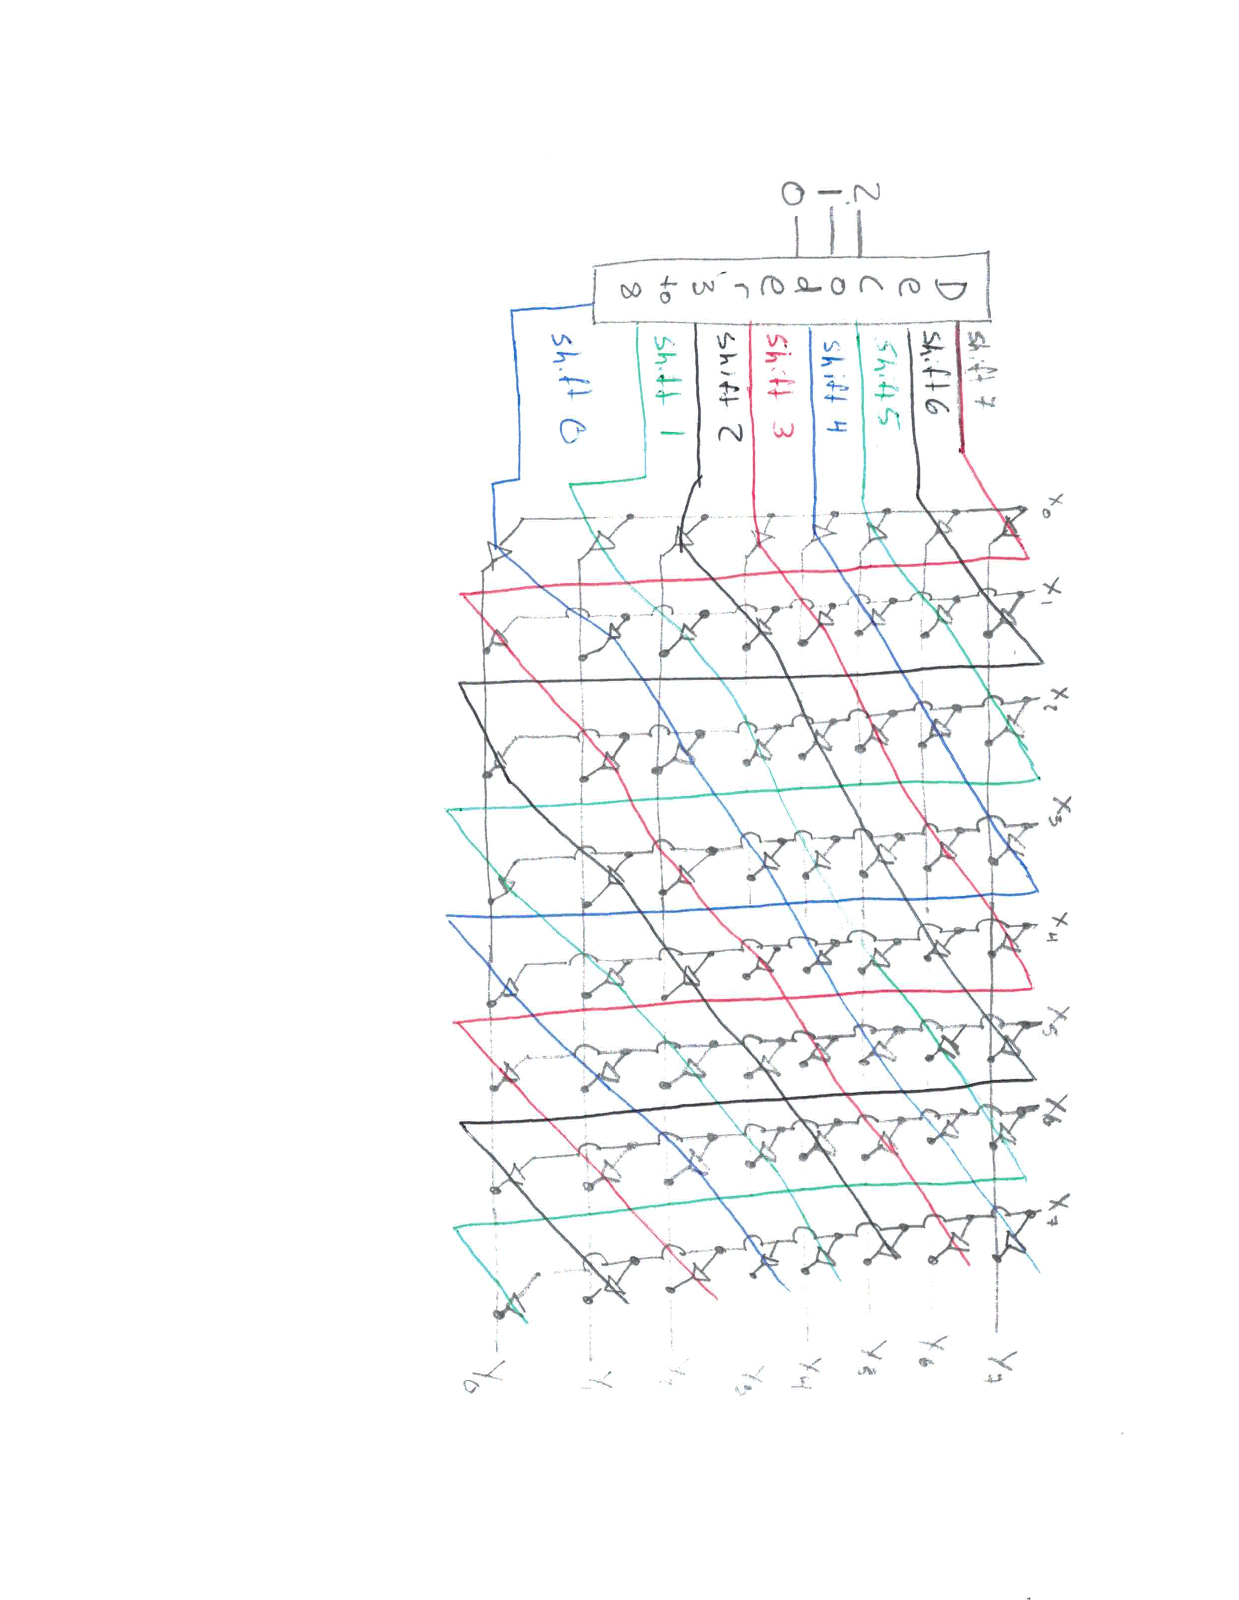
\includepdf[pages={1}]{BRN30055C8F6EB0_000502.pdf}
\newpage

		\begin{figure}[!ht]
 		 \caption{}
  		 \centering
    	 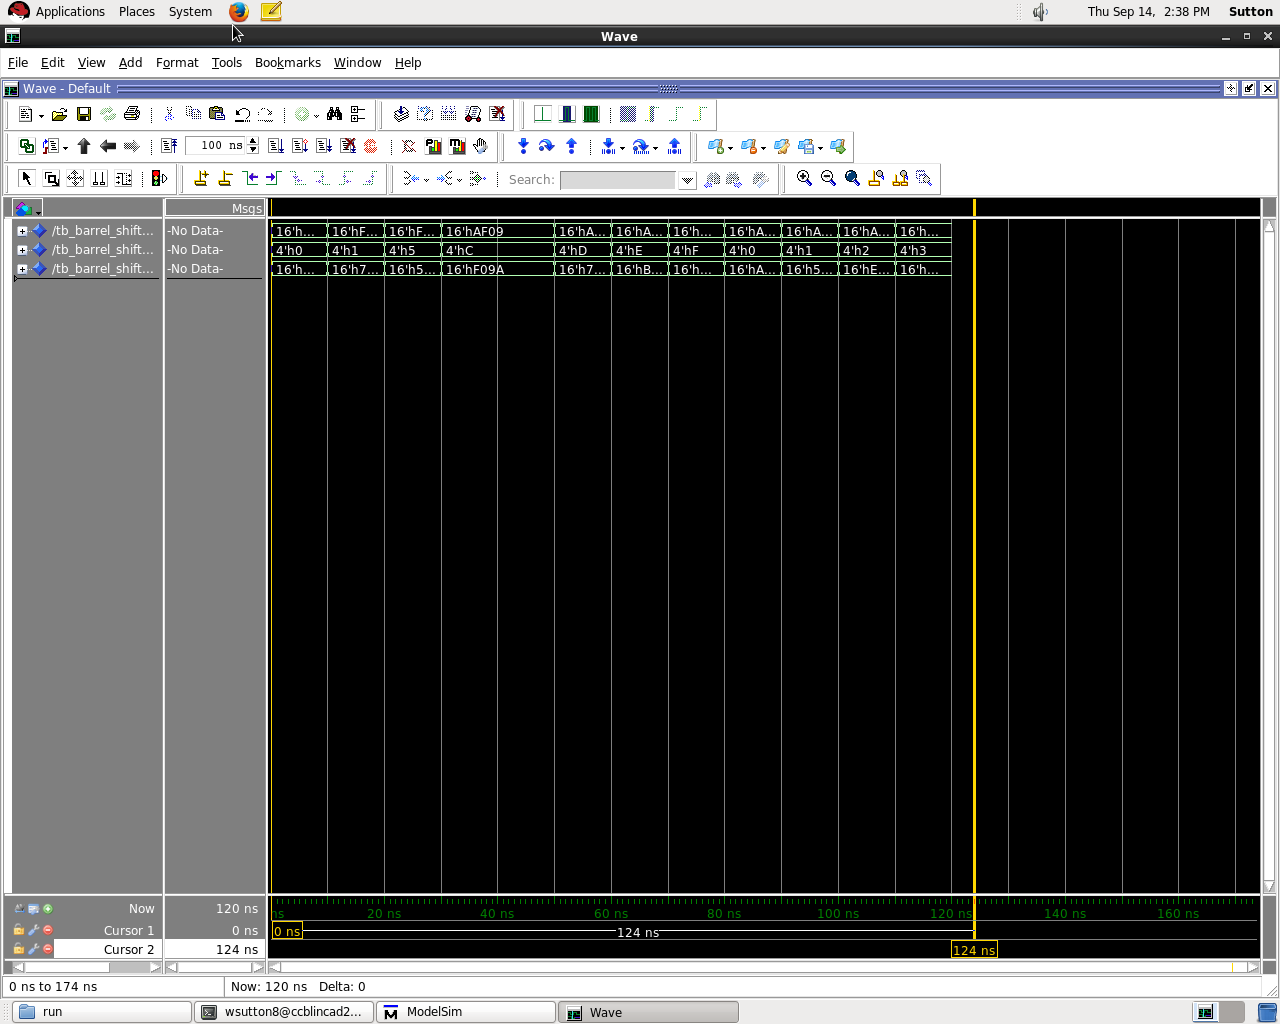
\includegraphics[width=1.2\textwidth]{Screenshot.png}
		\end{figure}
		\newpage
		
\section*{16Bit Design File}
\begin{lstlisting}
--Engineer     : Abhijit Gadad
--Date         : 8/25/2017
--Name of file : barrel_shifter_16.vhd
--Description  : implements a barrel shifter
--               of data width 8 bits

library ieee;
use ieee.std_logic_1164.all;
entity barrel_shifter is
--port list
    port(
         a   : in  std_logic_vector(15 downto 0); -- input data
         ctrl: in  std_logic_vector(3 downto 0); -- control word
         y   : out std_logic_vector(15 downto 0)  -- output data
        );
end barrel_shifter ;

architecture barrel_arch of barrel_shifter is
begin
--Comb logic which implements 
--the simple functionality
    with ctrl select
        y <= a                     when "0000",
             a(0) & a(15 downto 1) when "0001",
             a(1 downto 0) & a(15 downto 2) when "0010",
             a(2 downto 0) & a(15 downto 3) when "0011",
             a(3 downto 0) & a(15 downto 4) when "0100",
             a(4 downto 0) & a(15 downto 5) when "0101",
             a(5 downto 0) & a(15 downto 6) when "0110",
             a(6 downto 0) & a(15 downto 7) when "0111",
             a(7 downto 0) & a(15 downto 8) when "1000",
             a(8 downto 0) & a(15 downto 9) when "1001",
             a(9 downto 0) & a(15 downto 10) when "1010",
             a(10 downto 0) & a(15 downto 11) when "1011",
             a(11 downto 0) & a(15 downto 12) when "1100",
             a(12 downto 0) & a(15 downto 13) when "1101",
             a(13 downto 0) & a(15 downto 14) when "1110",
             a(14 downto 0) & a(15)          when others;

end barrel_arch; 
\end{lstlisting}
		
		
\section*{Comparison of 8 and 16 Bit barrel shifters}

\begin{tabular}{lll}
	 & 8Bit & 16Bit\\
	Resources (Slice LUTs) & 12 & 32\\
	Resources (Bonded IO Buffers) & 19 & 36\\
	Resources (Primitives LUT6) & 8 & 32\\
	Resources (Primitives INBUF) & 11 & 20\\
	Resources (Primitives IBUFCTL) & 11 & 20\\
	Resources (Primitives OBUF) & 8 & 16\\
	Power Usage (Total) & 6.051 & 12.015 \\
	Power Usage (Dynamic) & 4.647 & 10.502 \\
	Power Usage (Static) & 1.405 & 1.513 \\
\end{tabular}

\end{document}
